\documentclass[sigconf, nonacm]{acmart}
%\usepackage{cite}
\usepackage{amsmath,amsfonts}
\usepackage[ruled,linesnumbered,noend]{algorithm2e}
\usepackage{graphicx}
\usepackage{epstopdf}
\usepackage{textcomp}
\usepackage{xcolor}
\usepackage{xspace}
%\usepackage[draft]{hyperref}


\newcommand\vldbdoi{XX.XX/XXX.XX}
\newcommand\vldbpages{XXX-XXX}
% issue-specific
\newcommand\vldbvolume{14}
\newcommand\vldbissue{1}
\newcommand\vldbyear{2020}
% should be fine as it is
\newcommand\vldbauthors{\authors}
\newcommand\vldbtitle{\shorttitle}
% leave empty if no availability url should be set
\newcommand\vldbavailabilityurl{URL_TO_YOUR_ARTIFACTS}
% whether page numbers should be shown or not, use 'plain' for review versions, 'empty' for camera ready
\newcommand\vldbpagestyle{plain}

\newcommand\FIXME[1]{\textcolor{red}{FIX:}\textcolor{red}{#1}}
\newcommand\mypara[1]{\vspace{1.5mm}\noindent \textbf{#1}}
\newcommand\cparagraph[1]{\vspace{1.5mm}\noindent \textbf{#1}}
\definecolor{Gray}{gray}{0.95}


\newcommand\RV[1]{\textcolor{blue}{#1}}
\newcommand\SystemName{\textsc{Geneva}\xspace}
%subGraph sEarch usiNg parallEl Vertex mAtching
%\hypersetup{draft}




\begin{document}


\title{Fast GPU-based Subgraph Search Using Parallel Vertex Matching}

\author{Gangzhao Lu}
\affiliation{
	\institution{Harbin Institute of Technology}
	\city{Harbin}
	\state{China}
	\postcode{150001}
}
\email{lugangzhao@hit.edu.cn}

\author{Weizhe Zhang}
\affiliation{
	\institution{Harbin Institute of Technology}
	\city{Harbin}
	\state{China}
	\postcode{150001}
}
\email{wzzhang@hit.edu.cn}

\author{Xiao Sun}
\affiliation{
	\institution{Harbin Institute of Technology}
	\city{Harbin}
	\state{China}
	\postcode{150000}
}
\email{xiaosun@stu.hit.edu.cn}

\author{Meng Hao}
\affiliation{
	\institution{Harbin Institute of Technology}
	\city{Harbin}
	\state{China}
	\postcode{150001}
} \email{haomeng@hit.edu.cn}

\author{Zheng Wang}
\affiliation{
	\institution{University of Leeds}
	\city{Leeds}
	\state{United Kingdom}
	\postcode{LS2 9JT}
}
\email{z.wang5@leeds.ac.uk}



\begin{abstract}
Many graph-based workloads require performing \emph{subgraph matching} by finding all subgraphs of a data graph that are isomorphic to a
input query graph. Doing so on a real-life data graph is often computation-intensive because of the large number of graph vertices to be
examined. Existing schemes for subgraph matching all adopt a simple scheme by matching vertices of a query graph one by one. This
strategy fails to capitalize on the structure parallelism of graphs and can incur extensive memory accesses on GPUs. This work presents
\SystemName, a new GPU-based subgraph matching scheme that can match multiple query vertices simultaneously. Unlike prior work,
\SystemName performs subgraph matching within a single GPU kernel, eliminating many memory access operations required to process the
intermediate results. \SystemName also provides an enhanced storage format to reduce the memory footprint of graph data and improve
processing efficiency. We evaluate our approach by applying it to eight real-life graph datasets on an NVIDIA 2080Ti GPU. Experimental
results show that our approach improves GSI, the state-of-the-art graph matching framework, by 80\% on average (up to 96\%),
while reducing the memory footprint by 83\%.


%Subgraph search finds all subgraphs of a data graph that are isomorphic to a query graph. It is a fundamental operation in many application
%fields like analysis of protein-protein interaction network and community detection. Existing works adopt a simple search procedure that
%matches vertices of a query graph one by one, which incurs a large number of memory accesses during reading and writing intermediate
%results. In this work, we perform subGraph sEarch usiNg parallEl Vertex mAtching (\SystemName). Specifically, \SystemName can match as many
%query vertices as possible at each iteration and generate corresponding results in one GPU kernel. Compared to GSI, which is the
%state-of-the-art GPU-based subgraph search method, our approach achieves an average speedup of $5\times$. Additionally, we optimize the
%data graph format of GSI by replacing its hash indexes with interval indexes. The proposed interval-index format reduces the space cost and
%searching time of hash-index format by 83\% and 58\% respectively. To validate the effectiveness of parallel vertex matching, we also
%compare it to the single vertex matching devised based on our  parallel vertex matching. Results show that our approach improves the single
%vertex matching by 15.9\% on average.

%Based on properties of the data graph, there are many types of subgraph matching. In this work, we focus on matching query graphs on a labeled undirected data graph with the acceleration of GPU.
\end{abstract}

\maketitle
%%% do not modify the following VLDB block %%
%%% VLDB block start %%%
\pagestyle{\vldbpagestyle}
\begingroup\small\noindent\raggedright\textbf{PVLDB Reference Format:}\\
\vldbauthors. \vldbtitle. PVLDB, \vldbvolume(\vldbissue): \vldbpages, \vldbyear.\\
\href{https://doi.org/\vldbdoi}{doi:\vldbdoi}
\endgroup
\begingroup
\renewcommand\thefootnote{}\footnote{\noindent
This work is licensed under the Creative Commons BY-NC-ND 4.0 International License. Visit \url{https://creativecommons.org/licenses/by-nc-nd/4.0/} to view a copy of this license. For any use beyond those covered by this license, obtain permission by emailing \href{mailto:info@vldb.org}{info@vldb.org}. Copyright is held by the owner/author(s). Publication rights licensed to the VLDB Endowment. \\
\raggedright Proceedings of the VLDB Endowment, Vol. \vldbvolume, No. \vldbissue\ %
ISSN 2150-8097. \\
\href{https://doi.org/\vldbdoi}{doi:\vldbdoi} \\
}\addtocounter{footnote}{-1}\endgroup

%\ifdefempty{\vldbavailabilityurl}{}{
%\vspace{.3cm}
%\begingroup\small\noindent\raggedright\textbf{PVLDB Artifact Availability:}\\
%The source code, data, and/or other artifacts have been made available at \url{\vldbavailabilityurl}.
%\endgroup
%}
%%% VLDB block end %%%


\section{Introduction}
%Various areas, including social networks, chemical compounds, graph neural networks, and citation networks, use graphs as their underlying data structure. With the widespread adoption of graphs and the increasing graph size, many algorithms have been proposed to analyze graphs efficiently. Among these algorithms, subgraph search has always played an essential role in graph data mining.
%
%The goal of subgraph search is to find all subgraphs in a data graph $G$ that are isomorphic to a given query graph $q$. Though the problem
%is NP-complete, many approaches
%\cite{bhattarai2019ceci,guo2020gpu,tran2015fast,shi2020graphpi,bi2016efficient,zeng2020gsi,sun2020subgraph,guo2020exploiting,sun2020rapidmatch,lin2016network}
%have been proposed to speed up subgraph search in recent years. All these approaches adopt a similar 3-step procedure. They first build
%candidate sets and auxiliary data for query vertices, then generate a matching order for query vertices based on candidate sets and
%auxiliary data and finally match $q$ in $G$ according to the matching order. Most previous works mainly focus on generating an effective
%matching order that can reduce the number of intermediate results during subgraph search. For example, the main idea of the matching order
%generation algorithm proposed in \cite{bi2016efficient} is to match all non-tree edges regarding any spanning tree of $q$ as soon as
%possible to eliminate invalid subgraph candidates in the early stages of the matching process. We borrow this idea when designing our
%matching order generation algorithm.
%
%Some works \cite{lin2016network,guo2020gpu,tran2015fast,zeng2020gsi,guo2020exploiting} focus on optimizing subgraph search on GPUs, and GSI
%\cite{zeng2020gsi} achieves the best performance among all these approaches. GSI designs an edge label partitioned CSR (PCSR) format for a
%data graph to speed up accessing vertex neighbors. To build a PCSR format for a data graph, GSI first groups edges and corresponding
%vertices by the edge label into edge label partitions. Then, GSI builds a GPU-based CSR format for each edge label partition, which is the
%PCSR format. In order to find the position of a given vertex ID (VID) in PCSR, GSI adopts a hash function to map VIDs to positions
%(hash-PCSR), which needs many empty entries to reduce collisions (GSI uses 30 empty entries for each VID). In our approach, we also utilize
%PCSR format but replace the hash function with interval indexes (interval-PCSR). Additionally, we design a VID mapping algorithm for
%vertices in $G$ to map old VIDs to new VIDs, which can create more contiguous VIDs in each edge label partition and hence reduce the number
%of intervals. GSI proposes a Prealloc-Combine approach to make the parallel write of intermediate results more efficient. Nevertheless,
%this approach needs to launch two extra GPU kernels to write intermediate results to the right place. Unlike GSI, we utilize atomic
%operations inside the GPU kernel to calculate right positions for intermediate results. Therefore, we do not need extra GPU kernels.

Subgraph matching is a fundamental task of graph analysis. It requires finding all subgraphs from a data graph $G$ that are isomorphic to a
query graph $q$. Subgraph matching requires finding all the isomorphic subgraphs (known as graph embeddings) from the data graph $G$ by
ensuring both the vertex and the edge labels of the extract subgraph matches the vertex and edge labels of the query graph $q$. This
technique has a wide range of applications, including social network analysis \cite{wang2012truss,kairam2012The}, and chemical compound
search \cite{wooyoung2011Biological}.

Subgraph matching is an NP-complete problem \cite{garey1979Computers}, requiring significant computation time when processing large, real-life
graphs. A wide range of approaches have been proposed to speed up subgraph search
\cite{bhattarai2019ceci,guo2020gpu,tran2015fast,shi2020graphpi,bi2016efficient,zeng2020gsi,sun2020subgraph,guo2020exploiting,sun2020rapidmatch,lin2016network}.
These approaches adopt a typical 3-step process for subgraph matching. For the vertices in the query graph $q$, this process first builds
candidate sets and auxiliary data from the data graph $G$. It then determines a matching order that determines how each query vertex
should be matched from the candidate sets and auxiliary data before performing the graph matching by following the matching order.

Some of the most recent works attempt to leverage the GPU computation power for fast graph matching
\cite{lin2016network,guo2020gpu,tran2015fast,zeng2020gsi,guo2020exploiting}. GSI is the current state-of-the-art GPU-based graph matching
algorithm \cite{zeng2020gsi}, delivering the best performance on some of the representative datasets. It introduces a dedicated graph
storage format to reduce the memory footprint and improve the performance for graph vertex matching. While promising, existing approaches
can only match one vertex from the query graph in one go. Such a strategy leads to extensive GPU memory accesses because they need to load
and store the intermediate results for each vertex matching. These memory operations are expensive on GPUs with sizeable intermediate
results, which should be avoided if possible.


Most subgraph matching approaches do not explore data parallelism within a parallel thread because each thread only matches one vertex from
the query graph in each iteration. Such a strategy leads to extensive GPU memory accesses because the GPU worker needs to load and store
the intermediate results for each matched vertex. As we will show later in the paper, these memory operations are expensive on GPUs with
sizeable intermediate results, leaving much room for performance improvement. While there are techniques for reducing the intermediate
results on multi-core CPUs by simultaneously processing multiple graph edges \cite{lai2015scalable}, their strategy can handle a small set
of vertice matching patterns. Our work aims to close this gap by enabling the simultaneous process of multiple vertices in one go to reduce
the GPU memory accesses.

We propose \SystemName\footnote{\SystemName = subGraph sEarch usiNg parallEl Vertex mAtching.}, a new GPU-based subgraph matching framework
for parallel vertex matching within a GPU worker. \SystemName aims to match multiple vertices at each iteration and produce the
corresponding results in one GPU kernel. Unlike prior work \cite{lai2015scalable}, our approach support seven representative matching
patterns (Figure \ref{fig:matchpattern}). It uses one single GPU kernel to match multiple edges in a single GPU kernel simultaneously. By
matching multiple vertices and edges in a single GPU kernel, our approach eliminates the expensive GPU global memory addresses. \SystemName
provides new optimizing algorithms to generate the vertex matching order and process the commonly used matching pattern. \SystemName also
introduces a new graph storage format, which gives significant benefits for graph data storage overhead and processing time over
GSI.

We evaluate \SystemName by applying it to eight real-world data graphs on an NVIDIA 2080Ti GPU. We compare \SystemName against GSI, the
state-of-the-art GPU-based subgraph matching framework. Experimental results show that \SystemName reduces the processing time by $5\times$
on average over GSI. It uses 83\% less memory for graph data storage and improves the vertex search time by 58\%.




%All the abovementioned works match vertices of $q$ one by one, and thus need to write the intermediate results after matching one vertex
%and read the same intermediate results before matching the next vertex. The write and read operations are time-consuming, especially when
%the size of intermediate results is significant. To mitigate the cost of write and read operations, Lai et al. \cite{lai2015scalable}
%utilize MapReduce to implement a double-edge extension method. Their approach iteratively matches the query graph by a TwinTwig that
%consists of one edge (matching pattern 0 in Figure \ref{fig:matchpattern}) or two incident edges of a vertex (matching patterns 1 and 3 in
%Figure \ref{fig:matchpattern}). However, there are three inherent limitations in \cite{lai2015scalable}. First, edges in a TwinTwig must
%grow from the same vertex, which means their approach can not handle matching patterns 2, 4, and 7 in Figure \ref{fig:matchpattern}.
%Second, a TwinTwig contains at most two edges, but more than two edges can be processed at the same time, like matching patterns 5 and 6.
%Third, they use a simple method to generate results for matching pattern 1, which causes a number of unnecessary memory accesses to
%neighbors.

%To overcome limitations of \cite{lai2015scalable}, we propose an approach that performs subGraph sEarch usiNg parallEl Vertex mAtching
%(\SystemName).  Specifically, \SystemName matches as many query vertices as possible at each iteration and generate corresponding results
%in one GPU kernel. First, our approach can match vertices from different source vertices, e.g., matching patterns 2 and 4. Second, our
%approach can match as many edges as possible in a single GPU kernel (illustrated in Section \ref{sec:eliphase}). Third, we design an
%optimized algorithm (Algorithm \ref{algo:optDV}) to reduce unnecessary memory accesses for matching pattern 1. Moreover, we develop a new
%matching order generation algorithm (Algorithm \ref{algo:genmatchorder}) that is designed specifically for \SystemName. In summary, our
%approach can handle all matching patterns in Figure \ref{fig:matchpattern}.


This paper makes the following technical contributions:
 \begin{itemize}
\item It presents a novel parallel vertex matching method to support the process of multiple query vertices at the same time to reduce
    the GPU global memory access operations (Section \ref {sec:overview});
\item It presents an enhanced storage format to improve the storage efficiency and reduce the vertex search time (Section
    \ref{sec:storage});
\item It introduces an enhanced matching order generation algorithm to produce an appropriate vertex matching order to support efficient
    subgraph matching (Section \ref {sec:matchingorder}).
\end{itemize}


% We validate our approach from three aspects: (1) We obtain an average speedup of $5\times$ over GSI for subgraph search; (2) Experimental
% results show that our enhanced storage format significantly reduces the space cost and searching time of the storage format of GSI by 83\%
% and 58\% respectively; (3) Compared to the single vertex matching , which is modified based on our parallel vertex matching, our approach
% reduces the search time by 15.9\% on average.

% To summarize, we make the following contributions:
% \begin{itemize}
%    \item We propose a parallel vertex matching method that can match as many query vertices as possible to reduce the number of read and write operations of intermediate results.
%    \item We propose an enhanced storage format and a vertex ID mapping algorithm, which significantly reduces the space cost and searching time of the storage format of GSI.
%    \item We propose a new matching order generation algorithm and a new parallel write scheme to accommodate \SystemName.
%\end{itemize}

\section{Background}
\subsection{Preliminaries}
Given two graphs $q$ and $G$, the task of subgraph matching is to determine if the larger graph $G$ contains a subgraph that is isomorphic
to the query graph $q$. If the graphs include node and edge labels (or features), both the topology and the features should be matched. The
large graph $G$ is known as a data or target graph.  Subgraph matching is to find all subgraphs (also known as embeddings\footnote{Not to
confuse with the concept of embeddings (i.e., vectors) used by deep learning.} ) of the data graph, which are isomorphic to the query
graph.

In this work, we focus on mining subgraphs from an undirected labeled data graph $G=\{V,E,\Sigma,L_V,L_E\}$, where $V$, $E$ and $\Sigma$
are a set of vertices, edges and labels respectively,  $L_V$ is a function that associates a vertex $v \in V$ with a label $L_V \in
\Sigma$, and $L_E$ is a function that associates an edge $e \in E$ with a label $L_E \in \Sigma$. We describes a few important concepts of
subgraph matching as follows.


%\cparagraph{Subgraph matching.} A graph $g=\{V_g,E_g,\Sigma_g,L_{V_g},L_{E_g}\}$ is isomorphic to a query graph
%$q=\{V_q,E_q,\Sigma_q,L_{V_q},L_{E_q}\}$, if and only if there exists a bijective function $f: V_q \rightarrow V_g$ such that (1) $\forall
%u \in V_q$, $f(u) \in V_g$ and $L_{V_q}(u) = L_{V_g}(f(u))$; and (2) $\forall e_q=(u,u') \in E_q$, $e_g=(f(u),f(u')) \in E_g$ and
%$L_{E_q}(e_q)=L_{E_g}(e_g)$. Subgraph matching is to find all subgraphs (called embeddings) of a data graph $G$ that are isomorphic to a
%query graph $q$.

\cparagraph{Matching order.} Given a query graph $q$, a matching order $\pi$ is a permutation of vertices in $q$, where $\pi[i]$ is the
$i$th vertex in $\pi$. In essence, the matching order defines which order we match individual vertices of the query graph $q$ with the
counterparts from the data graph $G$. Studies have shown that choosing the right matching order can have a significant impact on
performance \cite{bi2016efficient,sun2020subgraph,sun2020rapidmatch,guo2020gpu}.  \SystemName provides a dedicated algorithm to generate
the matching order; see Section \ref {sec:matchingorder}.

\cparagraph{Partial embedding.} Given a query graph $q$ and a matching order $\pi$, \SystemName iteratively chooses unprocessed one or
multiple vertices from the matching order $\pi$ to perform subgraph matching. Until we iterate over all vertices from the query graph in
the match order, we only apply a sub-query graph and hence will only obtain a partial embedding (or subgraph). Our current implementation
matches up to two vertices at the same time, but the techniques can be extended to more than two vertices.

%Given a query graph $q$ and a matching order $\pi$, the subgraph matching will match one or two query
%vertices along $\pi$ iteratively. Before reaching the end of $\pi$, the matched query vertices and edges constitute a sub-query graph of
%$q$, which we call the partial query. The subgraphs of a data graph $G$ that are isomorphic to the partial query are called partial
%embeddings.

\cparagraph{Backward edge.} Given a query graph $q$ and a subgraph $q'$ of $q$, if an edge $e$ exists in $q$ but not in subgraph $q'$ and
$e$ connects two vertices of $q'$, we call $e$ the backward edge.

\begin{figure}[t!]
\centering
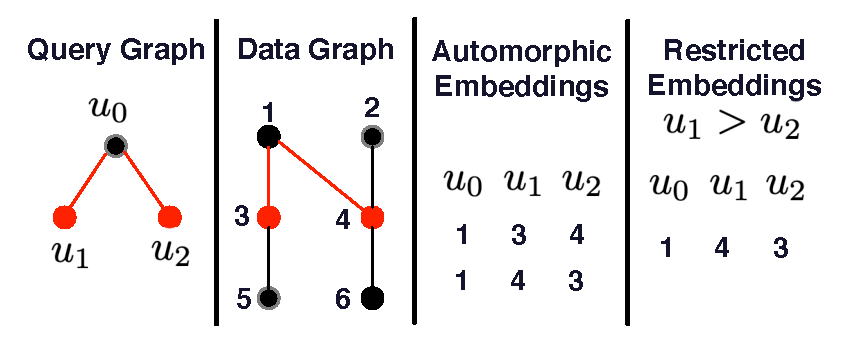
\includegraphics[width=\columnwidth]{./figure/automorphism.eps}
\caption{Examples of automorphic and non-automorphic embeddings.}	
\label{fig:automo}
\FIXME{Labeling the subgraphs.}
\end{figure}

\cparagraph{Handling graph symmetry.} For a symmetric query graph\FIXME{\cite{}}, multiple embeddings can be isomorphic to the same
subgraph of the data graph. Figure \ref{fig:automo} shows one of such examples, where the query graph has two symmetric vertices, $u_1$ and
$u_2$ and two isomorphic embeddings (Figure \ref{fig:automo}c) that all corresponding to the same subgraph of the data graph with vertices
$1, 3, 4$ (Figure \ref{fig:automo}b). To eliminate the duplicate embeddings, it is standard practice is to impose some restrictions on
graph matching \cite{ mawhirter2019graphzero, shi2020graphpi}. Figure \ref{fig:automo}d shows the matching criterion used by GraphPi and
GraphZero, which chooses an embedding that is \FIXME{describe the relation}. \SystemName uses the same criteria as GraphPi and GraphZero to
break the symmetry of a query graph.

%If a query graph is symmetric, multiple embeddings can be isomorphic to the same subgraph of the data graph. As shown in Figure
%\ref{fig:automo}, the query graph has two symmetric vertices, $u_1$ and $u_2$ and two isomorphic embeddings. We can see in Figure
%\ref{fig:automo} that the two embeddings are the same subgraph of the data graph. To eliminate redundant embeddings, GraphPi
%\cite{shi2020graphpi} and GraphZero \cite{mawhirter2019graphzero} generate restrictions on query vertices and the corresponding data
%vertices in each embedding. Figure \ref{fig:automo} shows that with the restriction $u_1 > u_2$, we can eliminate the redundant embedding.
%We use the same method as GraphPi and GraphZero to break the symmetry of a query graph.

\subsection{GPU Architecture}
GPUs are general-purpose massively parallel computing devices. They are widely used to accelerate graph processing tasks, including
subgraph matching \FIXME{\cite{}}. GPU processing units can be abstracted into a two-level hierarchy, the Streaming Multiprocessors (SMs)
and computing cores inside the SM. An SM is further divided into processing blocks. Each processing block contains a fixed number of
threads, called a warp that is the basic scheduling unit.

Modern GPUs also organize their memory into a hierarchical system, containing the global memory, a configurable shared memory, registers,
and potentially an L2 cache between the global memory and the shared memory. The thread-local registers are the fastest memory component,
having the lowest access latency (1-2 cycles). The SM local L1 caches and shared memory provide a larger storage capacity over the
thread-local registers but have modestly higher accessing latency of around 30 cycles. Like the RAM in a CPU system, the GPU’s off-chip
global memory provides the largest memory storage capacity on the GPU but has the most expensive accessing latency of around 500 cycles.

The NVIDIA CUDA programming model provides atomic functions to perform a read-modify-write atomic operation on one 32-bit or 64-bit word
residing in global or shared memory. In this work, we use the CUDA $atomicAdd$ function. This function reads a variable in global memory
before adding a number to it and then writes the result back to the same address.



%GPU has been used in many areas to accelerate applications. The popularity of GPU is primarily attributed to its massive parallelism. To support such large-scale parallelism, GPU employs a complex execution pipeline and memory hierarchy. Modern GPUs usually consist of multiple Streaming Multiprocessors (SMs), and each SM contains multiple Single-Instruction-Multiple-Thread (SIMT) units. Threads in the same SIMT unit are called a warp, the smallest scheduling unit in GPU. The thread-local registers are the fastest memory component, having the lowest access latency (1-2 cycles). The SM local L1 caches and shared memory provide a larger storage capacity over the thread- local registers but have modestly higher accessing latency of around 30 cycles. The off-chip global memory, similar to the RAM in a CPU system, provides the largest memory storage capacity on the GPU but has the longest accessing latency of around 500 cycles.
%
%CUDA provides atomic functions to perform a read-modify-write atomic operation on one 32-bit or 64-bit word residing in global or shared memory. In this work, we use $atomicAdd$ function to read a variable in global memory and add a number to it, and write the result back to the same address.


\section{Approach Design}
In this section, we give a detailed description of our approach, which targets on utilizing GPU to match query graphs on labeled graphs.
\subsection{Approach Overview}
Before the matching process, we first convert the data graph into our specific format that is space efficient and query friendly. Note that the conversion only needs to do once. Then, we perform subgraph matching on GPU, as shown in Algorithm \ref{algo:submatch}. We first decompose the query graph into query phases based on its vertex and edge labels. In the meanwhile, we generate a matching order for query phases and restrictions on query vertices (line 1). All edges extended in a query phase have the same edge label since we load one edge label partition at each iteration (lines 2, 7).
%\RV{There are two types of query phases, \emph{extension phase} that contains one of extension patterns 0-7 (line 9), and \emph{elimination phase}. We use SV-phase and NV-phase to represent extension phases that contain extension pattern 0 and extension patterns 1-7, respectively}.
The elimination phase contains multiple backward edges for elimination (line 11). The first query phase of the matching order is used to generate initial embeddings. We use the same GPU kernel as the extension phase to generate initial embeddings (line 4). The main difference between the first query phase and the extension phase is that the source VIDs of the former one are from the edge label partition, while the later one are from previous embeddings. Finally, we use different GPU kernels to match different types of query phases (lines 10, 12), and output the final embeddings (line 13). In the following sections, we elaborate each step in detail.

\begin{algorithm}[t!]
\KwIn{the data graph in our format $G$, the query graph $q$}
\KwOut{Embeddings of $q$ $EMB$}
$\pi \leftarrow \textsc{GenMatchOrder}(q)$\;
Load the edge label partition $elp$ whose edge label is $\pi[0].edgeLabel$ from $G$ to GPU\;
Allocate all available GPU memory space to $newEMB$\;
$\textsc{ExtKernel}(elp,NULL,newEMB,\pi[0])$\;
$EMB \leftarrow newEMB$\;
\For{$i \leftarrow 1$ \KwTo $\pi .size$}{
	Load the edge label partition $elp$ whose edge label is $\pi[i].edgeLabel$ from $G$ to GPU\;
	Allocate all available GPU memory space to $newEMB$\;
	\If{$\pi[i]$ is an extension phase}{
		$\textsc{ExtGPUKernel}(elp,EMB,newEMB,\pi[i])$\;
	}
	\Else{
		$\textsc{EliGPUKernel}(elp,EMB,newEMB,\pi[i])$\;
	}
	$EMB \leftarrow newEMB$\;
}
\caption{\textsc{SubgraphMatching}}
\label{algo:submatch}
\end{algorithm}


\subsection{Data Graph Format}
\begin{figure*}
\centering
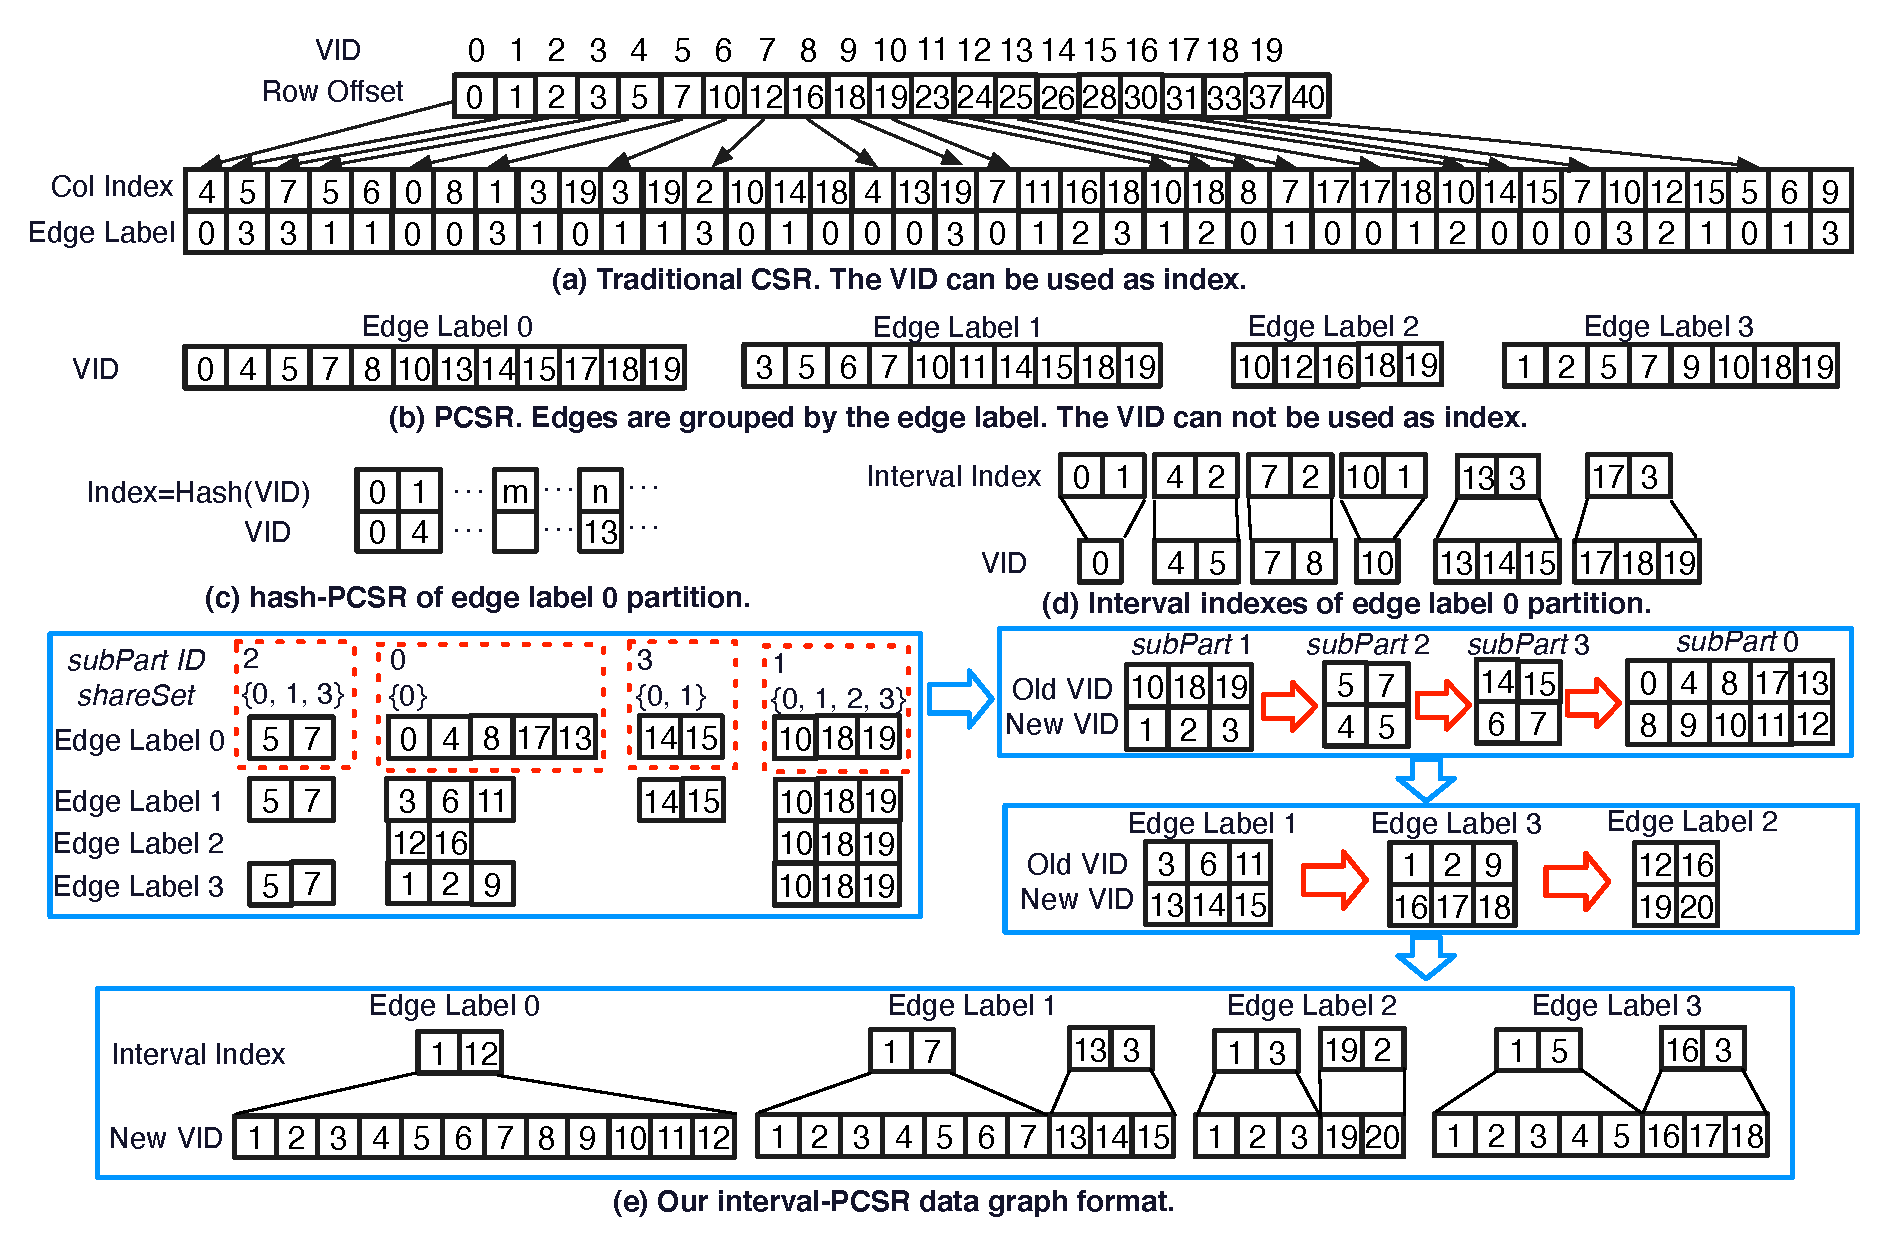
\includegraphics[width=\textwidth]{./figure/graphformat.eps}
\caption{Demonstration of data graph formats generated by traditional CSR, PCSR, hash-PCSR, non-optimized interval-PCSR, and our optimized interval-PCSR. Note that both non-optimized and optimized interval-PCSR do not need to store VIDs.}	
\label{fig:dataformat}
\end{figure*}

We first briefly describe the state-of-the-art data graph format for labeled graphs on GPU, hash-PCSR, which is proposed by GSI \cite{zeng2020gsi}. Then, we give a detailed illustration of our data graph format, interval-PCSR, which is more space and time efficient than hash-PCSR.
\subsubsection{hash-PCSR}
hash-PCSR groups edges of the same edge label into one edge label partition and builds the GPU-based CSR format for each edge label partition. Thus, only the partition that has the same edge label as the matching edge needs to be transferred to GPU memory, which significantly reduces the GPU memory consumption. In the traditional CSR format (Figure \ref{fig:dataformat}(a)), a VID can be used as the index to find the row offset of this vertex because VIDs in CSR are contiguous. However, VIDs may not be contiguous in an edge label partition (Figure \ref{fig:dataformat}(b)), and hence can not be used as the index. To overcome this problem, hash-PCSR designs a hash function to generate an index for each vertex based on its VID (Figure \ref{fig:dataformat}(c), this is a simplified hash-PCSR format, the detailed format is in \cite{zeng2020gsi}). To reduce collisions of the hash function, hash-PCSR uses 30 empty entries for each vertex and results in a large portion of unused GPU memory space.
\subsubsection{Our interval-PCSR}
\begin{algorithm}[t!]
\KwIn{the set of all edge label partitions $ELP$}
\KwOut{the mapping array $MAP$ with old and new vertex IDs are indices and values respectively}	
$newVID \leftarrow 1$\;
\While{ $ELP \neq \emptyset$ }{
	Choose the partition $elp \in ELP$ that has the most vertices\;
	Divide $elp$ into sub-partitions $subParts$\;
	\ForEach{$subPart \in subParts$}{
		Group IDs of partitions that contain $subPart$ into $shareSet$ and delete vertices of $subPart$ from these partitions\;
	}
	\While{$subParts \neq \emptyset$}{
		Choose the $subPart \in subParts$ that is shared by the most partitions and delete it from $subParts$\;
		Construct $MAP$ (assign new vertex IDs starting from $newVID$ to vertices in $subPart$ contiguously)\;
		$newVID \leftarrow newVID + subPart.size$\;
		$preSubPart \leftarrow subPart$\;
		\While{$preSubPart \neq \emptyset$}{
			Choose the $subPart \in subParts$ whose $shareSet$ has the most same partition IDs with the $shareSet$ of $preSubPart$ and delete the $subPart$ from $subParts$\;
			\If{Found the $subPart$}{
				Construct $MAP$\;
				$newVID \leftarrow newVID + subPart.size$\;
				$preSubPart \leftarrow subPart$\;
			}
			\Else{
				$preSubPart \leftarrow \emptyset$\;
				break\;
			}
		}
	}
	$ELP \leftarrow ELP/elp$\;
}
\caption{\textsc{GenMap}}
\label{algo:genmap}
\end{algorithm}

Our data graph format utilizes PCSR as the underlying data graph format but possesses efficient memory usage. To reduce the amount of unused memory space caused by the hash function, we leverage the interval index to represent contiguous VIDs in an edge label partition, as shown in Figure \ref{fig:dataformat}(d). Each interval index needs two entries to store the first VID and the length of this interval. The main issue of interval index format is that an edge label partition may contain numerous small intervals, which causes a number of memory accesses to find the right interval for a VID. For example, if we want to find the index of VID 7 in Figure \ref{fig:dataformat}(d), we need to compare 7 with the first three interval indexes and find VID 7 in the third interval index. With careful design, we can compare VID 7 only once to find its index. The key idea of our interval-PCSR is to design a mapping from original VIDs to new VIDs, which can generate more contiguous new VIDs in each edge label partition. Figure \ref{fig:dataformat}(e) and Algorithm \ref{algo:genmap} describe the workflow of our VID mapping process. The core design of our VID mapping algorithm can be explained by answering three questions:
\begin{itemize}
  \item[\emph{Q1:}] \emph{How to decide which partition should be assigned with new contiguous VIDs first?}\\We choose the partition that contains the most vertices (line 3) because the more vertices it contains, the higher probability it will be accessed. Therefore, reducing the number of intervals for this partition can help reduce the memory access latency. Figure \ref{fig:dataformat}(e) shows that edge label partition 0 is selected because it contains the most vertices.
  \item[\emph{Q2:}] \emph{How to decide which vertices of the partition should be assigned with new contiguous VIDs first?}\\We first group vertices shared by the same partitions into the same sub-partitions (line 4). After that, we only need to choose the best suitable sub-partition instead of vertices because vertices in a sub-partition can be assigned in any order without affecting the final interval index. For example, the edge label partition 0 in Figure \ref{fig:dataformat}(e) is divided into four sub-partitions. For $subPart$ 1, we can also map old VIDs 10, 18, and 19 to 2, 3, and 1, respectively, and the final interval index will still be the same. Then, we choose the sub-partition shared by the most partitions and assign its vertices with new VIDs contiguously (lines 8-10). The reason is that this kind of sub-partition has the most relations with other sub-partitions, and thus we try to assign contiguous VIDs to vertices in these related sub-partitions to reduce the total number of intervals. For example, in Figure \ref{fig:dataformat}(e), $subParts$ 1 and 2 are the most related sub-partitions. Thus we assign vertices in both sub-partitions contiguously, and all edge label partitions that contain both sub-partitions can represent them with one interval index.
  \item[\emph{Q3:}] \emph{How to decide which sub-partition should be processed next?}\\One or more partitions share the same sub-partition, and we call these partitions the $shareSet$ of the sub-partition (line 6). We intersect the $shareSet$ of each sub-partition with that of the previously selected sub-partition, and choose the sub-partition that has the largest intersection set (lines 13-20). In this way, we can assign contiguous VIDs to sub-partitions that exist in most partitions to reduce the number of interval indexes.
\end{itemize}

After replacing old VIDs with new VIDs, we build interval indexes, row offset, and column indexes for each edge label partition. Additionally, we group neighbors of each vertex by vertex labels and then sort neighbors in each group by their VIDs. To speed up the searching process of a VID, we load interval indexes of an edge label partition into GPU shared memory. In summary, our interval-PCSR is more space efficient than hash-PCSR in two aspects: (1) interval-PCSR does not need to store VIDs while hash-PCSR needs VIDs to evaluate whether the VID pointed by the hash index is the searching VID; (2) interval-PCSR has no empty entries while hash-PCSR uses 30 empty entries for each vertex to reduce collisions of the hash function.


\subsection{Extension Phase}
\begin{figure}
\centering
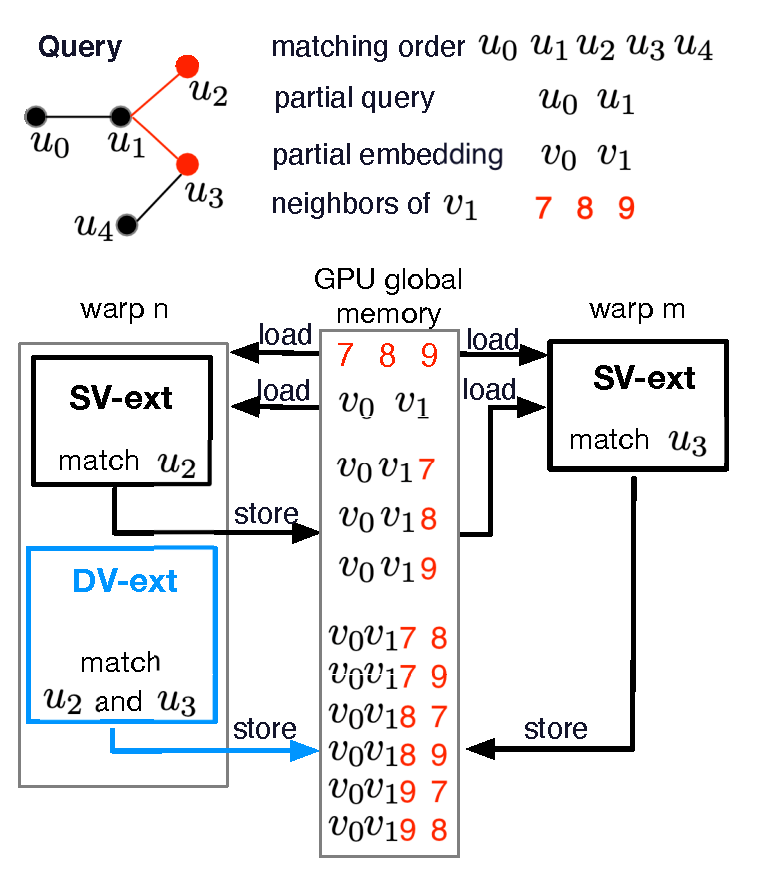
\includegraphics[width=0.9\columnwidth]{./figure/doubleext.eps}
\caption{Examples of single-vertex extension and our N-vertex extension methods.}	
\label{fig:doubleext}
\end{figure}
Previous works \cite{zeng2020gsi,sun2020subgraph} adopt the traditional single-vertex extension (SV-ext) method when matching the query graph in a data graph. However, this method ignores some critical information of the query graph when extending partial embeddings. In Figure \ref{fig:doubleext}, the SV-ext method needs to write intermediate results after matching $u_2$ and read intermediate results before matching $u_3$. This procedure is time-consuming because both write and read operations need to access GPU global memory. In order to speed up the matching process, \RV{we propose N-vertex extension (NV-ext) method that can extend partial embeddings with as many vertices as possible in one step. Our NV-ext method can handle all extension patterns shown in Figure \ref{fig:extpattern}}.


The main problem of subgraph matching on GPU is that the number of partial embeddings generated by each warp is different, thus we need to find the write address of new partial embeddings for each warp to avoid write conflicts. To solve this problem, GSI \cite{zeng2020gsi} uses a Prealloc-Combine method, which needs two extra GPU kernels and access all partial embeddings twice to find the write address for each warp. Though Prealloc-Combine method is more efficient than GpSM \cite{tran2015fast} which generates partial embeddings twice, it still incurs high memory overhead. Different from GSI, we use $atomicAdd$ inside the GPU kernel to calculate write addresses. The main performance issue of $atomicAdd$ is the sequential execution when multiple warps update the same variable at the same time. But this is not a severe problem in subgraph matching because of the intrinsic irregularity of subgraph matching.

\RV{Next, we give a detailed description of embedding generation algorithms  for extension patterns 0-4, and then demonstrate how to extend these algorithms to extension patterns 5-7.}

Algorithm \ref{algo:extphase} describes the overall workflow of generating embeddings for extension patterns 0-4. For each partial embedding (line 3), we first get source VIDs from the partial embedding according to the extension phase (line 4). Then, we search source VIDs in interval indexes and extract their neighbors (line 5).  Next, we remove invalid neighbors that have wrong vertex labels and do not satisfy restrictions. Finally, we use different algorithms to generate new embeddings for different extension patterns (lines 8-13).

\begin{algorithm}
\KwIn{the edge label partition $elp$, partial embeddings $EMB$, the starting address of new embeddings $newEMB$, the extension phase $extPhase$}
$count \leftarrow 0$\;
Load interval indexes of $elp$ into shared memory\;
\ForEach{$emb \in EMB$}{
	Get source VIDs $u_{s1}$ and $u_{s2}$ from $emb$\;
	Search $u_{s1}$ and $u_{s2}$ in interval indexes and extract their neighbors $ne1$ and $ne2$, respectively.\;
	Remove neighbors that do not have the same vertex labels as $u_{1}$ and $u_{2}$ from $ne1$ and $ne2$, respectively\;
	Remove neighbors that do not satisfy the restrictions of $u_{1}$ and $u_{2}$ from $ne1$ and $ne2$, respectively\;
	\If{$extPhase$ is extension pattern 1}{
		$\textsc{OptDouExt}(emb,ne1,count,newEMB)$\;
	}
	\ElseIf{$extPhase$ is one of extension patterns 2, 3, and 4}{
		$\textsc{DouExt}(emb,ne1,ne2,count,newEMB)$\;
	}
	\Else{
		We use the traditional SV-ext method to generate embeddings for $extPhase$\;
	}
}

\caption{\textsc{ExtPhaseKernel}}
\label{algo:extphase}
\end{algorithm}

For extension patterns 2-4, we devise a direct method, Algorithm \ref{algo:generalDV}, to generate new embeddings. The main idea of Algorithm \ref{algo:generalDV} is to iterate over all combinations of candidates of $u_{1}$ and $u_{2}$, denoted as $C_1$ and $C_2$ respectively, and construct new embeddings by appending each valid combination to a new copy of the current embedding $emb$. We say a combination is valid, if neither VIDs in the combination equals to VIDs in $emb$. To avoid checking this condition repeatedly, we first check this condition for all vertices in $C_2$ once (lines 3-4) and record indexes of vertices whose VIDs also exist in $emb$ (line 5). To fully utilize $C_2$, we generate new embeddings while checking the condition. Once a vertex in $C_2$ is checked valid (lines 6-7), we assign this vertex and the first valid vertex in $C_1$ to $u_2$ and $u_1$, respectively (lines 1,8). Then, we write the new partial embedding $(emb,u_1,u_2)$ to the corresponding address (lines 9-10).

\begin{algorithm}
	\KwIn{the partial embedding $emb$, candidates of $u_1$ $C_1$, candidates of $u_2$ $C_2$, the number of newly written embeddings $totNum$, the starting address of new embeddings $newEMB$}
	Find the index $i$ of the first valid vertex in $ne1$\;
	$writePos \leftarrow atomicAdd(totNum,1 \times C_{2}.size)$\;
	\For{$j \leftarrow 0$ \KwTo $C_{2}.size$}{
		\If{$C_2[j] \in emb$}{
			Add $j$ to the set $boundry$\;
			$u_1 \leftarrow 0$; $u_2 \leftarrow 0$\;
		}
		\Else{
			$u_1 \leftarrow C_1[i]$; $u_2 \leftarrow C_2[j]$\;
		}
		Write the new embedding ($emb$, $u_1$, $u_2$) to the address pointed by $newEMB+writePos$\;
		$writePos \leftarrow writePos + emb.size+2$\;
	}
	$i \leftarrow i+1$\;
	\While{$i < C_{1}.size$}{
		Load 32 candidates from $C_1$ into $tmp$; $i \leftarrow i+32$\;
		Remove candidates that exist in $emb$ from $tmp$\;
		$writePos \leftarrow atomicAdd(totNum,tmp.size \times (C_{2}.size-boundry.size))$\;
		\ForEach{$0 \leq k<tmp.size$ and $0 \leq j<C_{2}.size$ and $j \notin boundry$}{
			\If{This is EP 2 and $C_1[k]=C_2[j]$}{
				$u_1 \leftarrow 0$; $u_2 \leftarrow 0$\;
			}
			\Else{
				$u_1 \leftarrow C_1[k]$; $u_2 \leftarrow C_2[j]$\;
			}
			Write the new embedding ($emb$, $u_1$, $u_2$) to the address pointed by $newEMB+writePos$\;
			$writePos \leftarrow writePos + emb.size+2$\;
		}
	}
	\caption{\textsc{DouExt}}
	\label{algo:generalDV}
\end{algorithm}

At the beginning of Algorithm \ref{algo:generalDV}, we allocate space for new partial embeddings generated when checking conditions for $C_2$ (line 2). Since we do not know the number of valid vertices in $C_2$ until all vertices are checked, we use the vertex count of $C_2$, denoted as $C_{2}.size$, to overestimate the number of new partial embeddings. If there are invalid vertices in $C_2$, we assign 0 to $u_1$ and $u_2$ to indicate invalid partial embeddings (line 6). When a GPU kernel read a partial embedding that contains 0, it skips this partial embedding.

In Algorithm \ref{algo:generalDV}, after finding invalid vertices in $C_2$, we generate new partial embeddings for rest vertices in $C_1$ (lines 11-12). In each iteration, we load 32 vertices in $C_1$ into shared memory $tmp$ and remove invalid ones from $tmp$ (lines 13-14). In order to allocate space for new partial embeddings, we estimate its count as the number of combinations of $tmp$ and valid vertices in $C_2$ (line 15). Then, we generate new partial embeddings for these combinations (line 16). As $u_1$ and $u_2$ have the same vertex label in extension pattern 2, there is a chance that two candidates of $u_1$ and $u_2$ are equal (line 17), which makes the generated partial embedding invalid. Next, we assign 0 to $u_1$ and $u_2$ if the partial embedding is invalid (line18), otherwise assign corresponding candidates to $u_1$ and $u_2$ (line 20). Finally, write the new partial embedding to the specified address (lines 21-22).

However, Algorithm \ref{algo:generalDV} is not appropriate for extension pattern 1. In extension pattern 1, $u_1$ and $u_2$ are extended from the same source vertex $u_{s1}$ and have the same vertex label, thus $C_1 = C_2$. If Algorithm \ref{algo:generalDV} is applied to extension pattern 1, each vertex in $C_2$ can be accessed by up to $C_1.size$ times. As shown in the left part of Figure \ref{fig:ep1opt}, element 1 is accessed at each iteration of $i$. If $C_1.size>32$, we need to reload element 1 from global memory each time we access it. Other elements also encounter the same problem.

\begin{figure}
\centering
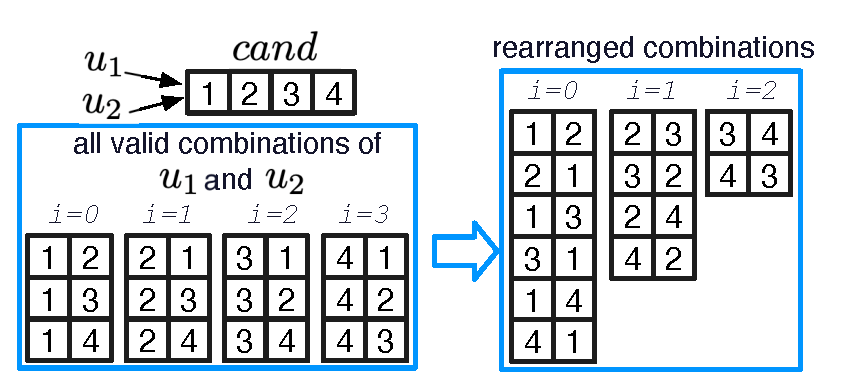
\includegraphics[width=\columnwidth]{./figure/ep1opt.eps}
\caption{An example of generating new embeddings for extension pattern 1.}	
\label{fig:ep1opt}
\end{figure}

To speed up the matching process of extension pattern 1, we rearrange the generation order of combinations, as shown in the right part of Figure \ref{fig:ep1opt}, to make accesses more register friendly. Algorithm \ref{algo:optDV} demonstrates the core design of the optimized generation method for extension pattern 1. From the right part of Figure \ref{fig:ep1opt}, we make two important observations to guide the design of Algorithm \ref{algo:optDV}. First, the element $C_1[i]$ is only used at iteration $i$ and thus we load it into a register (line 2) to reduce its access latency. Second, each time we generate a combination, we can reverse the combination to obtain another combination immediately without reloading data from global memory (lines 4-5).

\begin{algorithm}
	\KwIn{the partial embedding $emb$, candidates $C$, the number of newly written embeddings $totNum$, the starting address of new embeddings $newEMB$}
	$writePos \leftarrow atomicAdd(totNum,C.size \times (C.size-1))$\;
	\For{$i \leftarrow 0$ \KwTo $C.size-1$}{
		\For{$j \leftarrow i+1$ \KwTo $C.size$}{
			Write new embeddings ($emb$, $C[i]$, $C[j]$) and ($emb$, $C[j]$, $C[i]$) to the address pointed by $newEMB+writePos$\;
			$writePos \leftarrow writePos + (emb.size+2) \times 2$\;
		}
	}
	\caption{\textsc{OptDouExt}}
	\label{algo:optDV}
\end{algorithm}

Methods of generating partial embeddings for extension patterns 5-7 are illustrated in the following: (1) 

\subsection{Elimination Phase} \label{sec:eliphase}
GSI \cite{zeng2020gsi} matches only one query edge in a GPU kernel and Lai et al. \cite{lai2015scalable} matches at most two query edges at each iteration. Both methods can not fully utilize the elimination power of backward edges. In our approach, we match as many backward edges as possible to eliminate invalid partial embeddings at early stages. Algorithm \ref{algo:eliphase} demonstrates how our approach deals with the eliminate phase. For each partial embedding $emb$ (line 2), we first check if all query edges in the elimination phase can be matched in $emb$ (line 4). If so (line 5), we write $emb$ to the shared memory $tmp$ (line 6) and write $tmp$ to global memory if it is full (lines 7-9).
\begin{algorithm}
\KwIn{the edge label partition $elp$, partial embeddings $EMB$, the number of generted embeddings $totNum$, the elimination phase $eliPhase$}
Load interval indexes of $elp$ into shared memory\;
\ForEach{$emb \in EMB$}{
	\ForEach{$edge \in eliPhase$}{
		Check if there is an edge in $emb$ that can match $edge$\;
	}
	\If{all edges in $eliPhase$ are matched}{
		Write $emb$ to shared memory $tmp$\;
		\If{$tmp$ is full}{
			$writePos \leftarrow atomicAdd(totNum,tmp.size)$\;
			Write $tmp$ to the address pointed by $newEMB+writePos$\;
		}
	}
}
\caption{\textsc{EliPhaseKernel}}
\label{algo:eliphase}
\end{algorithm}



\subsection{Matching Order}
\begin{figure}
\centering
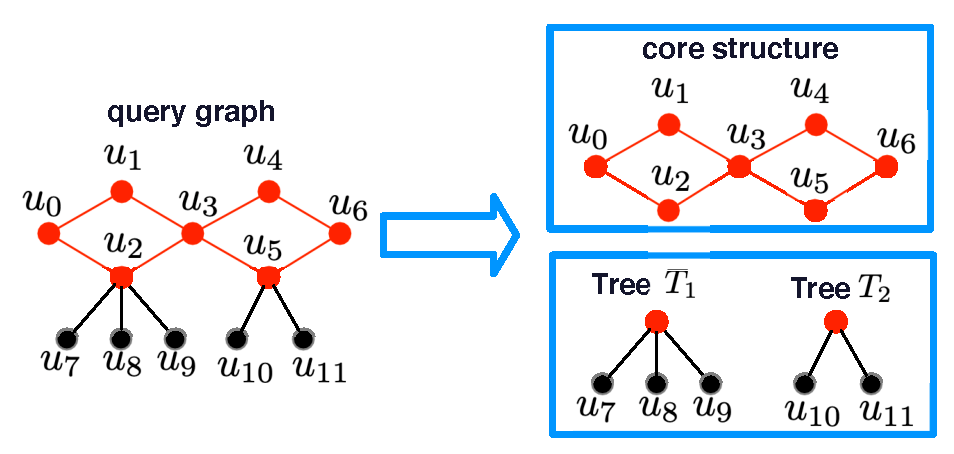
\includegraphics[width=\columnwidth]{./figure/genmatchorder.eps}
\caption{An illustration of how to decompose a query graph into a core structure and trees.}
\label{fig:matchorder}
\end{figure}
\RV{In this section, we first give a brief description of matching order generation method used in \cite{bi2016efficient}, and then demonstrate the details of our matching order generation algorithm based on NV-ext method.}

\RV{The main goal of \cite{bi2016efficient} is to match backward edges as soon as possible to eliminate invalid embeddings at early stages. Therefore, they generate a subgraph of $q$ that contains all backward edges regarding any spanning tree of $q$ by iteratively removing all degree-one vertices from $q$. The generated subgraph, which is called the core structure as shown in Figure \ref{fig:matchorder}, is matched first. In our approach, we also match the core structure first, and then the trees}.

\RV{When decomposing the core structure into extension and elimination phases, we need to adhere to an important constraint, which is that only extension patterns 0-4 can be used to decompose the core structure. The reason is explained as follows. In order to eliminate invalid embeddings as soon as possible, we need to first match circles in the core structure, which are \{$u_0$, $u_1$, $u_2$\} and \{$u_2$, $u_3$, $u_4$, $u_5$\} in Figure \ref{fig:matchorder}. Therefore, we need to extend at most two vertices when matching a circle because vertices have exactly two neighbors in a circle.}

\RV{For the core structure in Figure \ref{fig:matchorder}, we first use extension pattern 1 to match $u_0$, $u_1$, and $u_2$, then match the backward edge $(u_0, u_1)$. If we first match $u_0$, $u_1$, $u_2$, $u_4$, and $u_5$ with extension pattern 5, and then the backward edge $(u_0, u_1)$, a large number of invalid embeddings may be generated after matching the extension pattern 5, which significantly slows down the matching performance. After matching the core structure, we can use any appropriate extension patters to match trees. For example, extension patterns 5 and 1 can be used to match $T_1$ and $T_2$ in Figure \ref{fig:matchorder} respectively.}

%Many previous researches \cite{bi2016efficient,sun2020subgraph,sun2020rapidmatch,guo2020gpu} have explored how to generate an effective matching order to speed up the matching process. However, all of these methods are designed for single-vertex extension subgraph matching and not suitable for our DV-ext method. In this work, we propose a matching order generation algorithm based on the structural information of the query graph. The key idea of our algorithm is to match all available backward edges in the query graph as soon as possible to eliminate invalid partial embeddings at early stages. If no backward edges are available, we extend the partial query graph by one or two vertices. Algorithm \ref{algo:genmatchorder} demonstrates our matching order generation algorithm.
%When extending an edge that connects two matched query vertices, we can add a restriction on two matched query vertices, which is that the neighbors of one vertex must contain the other vertex. Thus, we can guarantee that the number of generated embeddings is less than or equal to the number of previous embeddings. Based on this observation,


\RV{Based on \cite{bi2016efficient} and our NV-ext method, we design Algorithm \ref{algo:genmatchorder} to generate matching order of query phases. At the beginning of Algorithm \ref{algo:genmatchorder}, we adopt methods proposed in \cite{shi2020graphpi,mawhirter2019graphzero} to generate restrictions on VIDs in partial embeddings (line 1). Thus, we can avoid generating invalid partial embeddings. Then we generate the core structure of $q$ by iteratively removing degree-one vertices from $q$, and construct trees of $q$ using removed vertices (line 2).}

\RV{In order to match the core structure, we first find the smallest circle in the core structure (line 3), and then select vertices in the circle that conform to the highest priority extension pattern among extension patterns 0, 1, and 3 (line 4). The selected vertices constitute the initial phase (lines 5-6), which is a special kind of extension phase. Different from the normal extension phase that fetches source vertices from partial embeddings, the initial phase fetches the source vertex from the edge label partition. After generating the initial phase, we iteratively find vertices in the circle that conform to extension patterns 0-4 and choose the one with the highest priority (lines 7-9). Finally, we use the backward edge in the circle to construct an elimination phase (line 10).}

\RV{After decomposing the smallest circle, we iteratively construct query phases for the rest vertices and edges in the core structure (line 11). First, we find all backward edges and group them by the edge label (lines 12-13). For each group, we construct an elimination phase (lines 14-15). If no backward edges are found, we search for unmatched vertices in the core structure that can form one of extension patterns 0-4, and choose the one with the highest priority (lines 16-18).}

\RV{After matching the core structure, we can use any appropriate one of extension patterns 0-7 to match rest vertices that are not in the core structure since there is no backward edge left. At each iteration, we find vertices that can form extension patterns 0-7 and select the one with the highest priority (lines 19-21).}
% Since more than one extension patterns may be found, we assign each extension pattern a priority and choose the extension pattern with the highest priority.
%\begin{itemize}
%  \item Assign the first priority to extension pattern 1. As $u_1$ and $u_2$ in extension 1 have the same vertex label and source vertex, candidate sets of both vertices are equal. Therefore we can generate new embeddings of extension pattern 1 efficiently with Algorithm \ref{algo:optDV}.
%  \item Assign the second priority to extension pattern 3. The candidate sets of $u_1$ and $u_2$ in extension pattern 3 are different but all belong to the neighbors of the same source vertex. Therefore, we only need to find the address of neighbors of the source vertex once and then find addresses of two vertex labels.
%  \item Assign the third priority to extension pattern 4. We need to find addresses of neighbors of two source vertices and then find addresses of two vertex labels in the corresponding neighbors. Moreover, the vertex labels of $u_1$ and $u_2$ are different, this pattern will not generate invalid embeddings.
%  \item Assign the fourth priority to extension pattern 2. We need to find addresses of neighbors of two source vertices and then find addresses of two vertex labels in the corresponding neighbors. As the vertex labels of $u_1$ and $u_2$ are the same, there may be same vertices in both candidate sets which can lead to invalid embeddings.
%\end{itemize}

% The main issue is that there may be more than one pairs of $u_1$ and $u_2$ can form the same extension pattern with the highest priority (line 17). In our approach, we choose the pair that has the most unmatched neighbors in the query graph (line 18). In this way we increase the chance to find backward edges and high priority extension patterns when constructing the next query phase.
 %Methods proposed in \cite{guo2020gpu, shi2020graphpi,bi2016efficient} use data graph information to assist the matching order generation. We leave this method for our future work.

\begin{algorithm}
	\KwIn{the query graph $q$}
	\KwOut{the match phase queue $matchPhase$}
	Generate restrictions to eliminate automorphisms\;
	Generate the core structure $C$ and trees $T$ of $q$\;
	Find the smallest circle $minc$ in $C$\;
	Select vertices in $minc$ that conform to extension patterns 0, 1, and 3, and choose the highest priority extension pattern\;
	Construct the initial phase with vertices corresponding to the selected extension pattern\;
	Add the initial phase to $matchPhase$\;
	\For{vertices in $minc$ that conform to extension patterns 0-4}{
		Choose the highest priority extension pattern and construct an extension phase\;
		Add the extension phase to $matchPhase$\;
	}
	Construct an elimination phase with the backward edge in $minc$ and add it to $matchPhase$\;
	\For{rest vertices and edges in $C$}{
		\If{there are backward edges}{
			Group all backward edges by the edge label\;
			\ForEach{group $g$}{
				Construct an elimination phase $eliPhase$ based on $g$ and add it to $matchPhase$\;
			}	
		}
		\Else{
			Find vertices that conform to extension patterns 0-4 and choose the one with the highest priority\;
			Construct an extension phase and add it to $matchPhase$\;
		}
	}
	\For{vertices in $T$}{
		Find vertices that can form extension patterns 0-7 and select the one with the highest priority\;
		Construct an extension phase and add it to $matchPhase$\;
	}
	\caption{genMatchOrder}
	\label{algo:genmatchorder}
\end{algorithm}

\subsection{Load Balance}
In GPU, once a thread block is scheduled to run on an SM, it will not be scheduled out until all warps in this thread block are finished. Therefore, if one warp matches a vertex or an edge that has many candidates, all warps in the same thread block have to wait for its completion. To address this problem, GSI designs a four-layer balance scheme. However, their scheme needs to invoke a GPU kernel inside a GPU kernel, which is time-consuming as illustrated in Section \ref{sec:compargsi}. Different from GSI, we use fixed warps, which means the maximum concurrent warps are generated and will not be scheduled out during execution, to perform subgraph matching. In this way, a warp with small workload can match next embedding without waiting for other warps. Only when there is no embeddings left, the faster warps have to wait for the slower warps. Our approach is simple yet effective, it can mitigate load imbalance to some extend. A more powerful load balance scheme can be designed and we leave this for a future study. 
\section{Experimental Setup}

\subsection{Hardware and Workloads}

\begin{table} [t!]
\centering
  \caption{Data graphs.}
  \label{tab:datagraph}
  \small
  \begin{tabular}{llllll}
  \toprule
    \textbf{Type of sizes}&\textbf{Graph Name} &$|V|$&$|E|$&$|L_V|$&$|L_E|$\\
    \midrule
    Tiny	&Enron		&36K	&183K	&3	&3 \\
    Tiny	&FirstMM 	&56K	&126K	&3	&3 \\
    Small	&DD			&0.3M	&0.8M	&5	&5\\
    Small	&Gowalla	&0.2M	&0.9M	&5	&5\\
    Medium	&Patents	&3.7M	&16M	&7	&7\\
    Medium	&Reddit		&4.6M	&5.5M	&7	&7\\
    Large	&Orkut		&3M		&117M	&12	&12\\
	Large	&sinaweibo	&58M	&261M	&12	&12\\

    \bottomrule
  \end{tabular}
\end{table}
\cparagraph{Experimental platform.} We evaluate our approach on a multi-core workstation with an NVIDIA RTX2080Ti GPU. The server has a
12-core Intel Xeon E5-2697 CPU at 2.3 GHz and 256 GB of RAM. The GPU has 11 GB of memory and 68 SMs where each SM has 4350 CUDA cores and
64KB of shared memory

\cparagraph{Data graphs.} We use eight real-world data graphs in our experiment. The size of the graphs ranges from tiny to large, as
illustrated in Table \ref{tab:datagraph}. Graphs Enron \cite{leskovec2009community}, Gowalla \cite{cho2011friendship}, Patents
\cite{leskovec2005graphs}, and Orkut \cite{yang2015defining} are obtained from the SNAP dataset \cite{snapnets}, while FirstMM, DD, Reddit,
and sinaweibo are obtained from the Network Repository \cite{ryan2015network,nr-sigkdd16}.

\cparagraph{Query graphs.} Like \FIXME{xx}, we use \FIXME{xx} different types of query graphs. \FIXME{Describe your query graphs here.}

\subsection{Evaluation Methodology}
\cparagraph{Competing methods.} We compare \SystemName against GSI \cite{zeng2020gsi}, the state-of-the-art GPU-based subgraph search
method. We also provide an implementation variant of \SystemName, which matches one vertex at a time. This SV-match scheme is implemented
by splitting each extension phase that contains one of matching patterns 1-7 in Figure \ref {fig:matchpattern} into multiple extension
phases that contain only the matching pattern 0.

\cparagraph{Performance report.} To measure the runtime of an approach, we run each test case at least five times and compute the 95\%
confidence interval bound. We increase the number of profiling runs if the interval is greater than 2\%. We then report the geometric mean
across runs.

\section{Experimental Results}
Overall, our interval-PCSR reduces the space cost of hash-PCSR by 83\% on average and achieves an average speedup of $2.4\times$ over hash-PCSR when performing VID search. Moreover, \SystemName achieves an average speedup of $5\times$ over GSI for the task of subgraph search. Experimental results show that our approach can significantly improve the performance of subgraph search on GPUs.

\subsection{Evaluation of Data Graph Formats}
In this section, we first present the space cost of three data graph formats, including CSR, hash-PCSR, and  interval-PCSR, and then the searching time of hash-PCSR and interval-PCSR.

The results of space cost are shown in Table \ref{tab:graphsize}. We can see from Table \ref{tab:graphsize} that CSR has the smallest space among three data graph formats. The reason is that all VIDs in CSR are contiguous and unique, while VIDs in PCSR are non-contiguous and many duplicate VIDs exist in different edge label partitions. However, we need to transfer the whole CSR format graph to GPU in order to perform subgraph search, which is space and time consuming. In contrast, our interval-PCSR achieves similar space cost as CSR but only needs to transfer one edge label partition to GPU before each iteration of subgraph search. AS shown in Table \ref{tab:graphsize}, the size of the maximum edge label partition in interval-PCSR (denoted as \emph{Max}) is greatly smaller than CSR, which makes data transfer in our approach more efficient.


\begin{table}
\centering
  \caption{Space overhead of CSR, hash-PCSR (GSI), and our interval-PCSR storage formats. The \emph{Max} column represents the size of maximum edge label partition in
  the interval-PCSR. The \emph{reduction over hash-PCSR} column represents the percentage of the space saved given by our interval-PCSR over GSI's hash-PCSR.}
  \label{tab:graphsize}
  \scriptsize
  \begin{tabular}{lllllr}
  \toprule
    \textbf{Graph} &\textbf{CSR}&\textbf{interval-PCSR}&\textbf{hash-PCSR}&\emph{\textbf{Max}}&\emph{Reduction over hash-PCSR}\\
    \midrule
    Enron 		&1.6MB	&1.7MB	&13MB	&0.6MB	&87\% \\
    FirstMM 	&1.2MB	&1.5MB	&22MB	&0.5MB	&93\% \\
    DD 			&15MB	&11MB	&139MB	&2.1MB	&87\% \\
    Gowalla 	&8.1MB	&9.4MB	&74MB	&1.9MB	&94\% \\
    Patents 	&149MB	&184MB	&1.6GB	&26MB	&89\% \\
    Reddit 		&60MB	&71MB	&901MB	&10MB	&92\% \\
    Orkut 		&906MB	&997MB	&1.94GB	&100MB	&50\% \\
    sinaweibo	&2.2GB	&2.5GB	&10GB	&256MB	&75\% \\

    \bottomrule
  \end{tabular}
\end{table}

Our interval-PCSR can averagely reduce the space cost of hash-PCSR by 83\%.The main reason for the large space cost of hash-PCSR is empty
entries in hash indexes. The hash-PCSR groups edges by their edge label, which makes VIDs in each group are non-contiguous. To find the
index of a given VID, hash-PCSR designs a hash function to map a given VID to a position that points to the neighbors of the VID. If
multiple VIDs are mapped to the same position, a sequential search has to be performed to find the true position of the VID, which is a
time-consuming operation in GPU. Therefore, hash-PCSR trades space for time and generates 30 empty entries for each VID to reduce
collisions. This method significantly reduces collisions and also incurs large space cost. For example, the largest edge label partition in
the data graph Enron contains 24737 VIDs. And hash-PCSR needs $32 \times 24737$ 32-bit variables to store hash indexes. While in our
interval-PCSR, we use one interval index to represent a range of contiguous VIDs and adopt Algorithm \ref{algo:genmap} to generate more
contiguous VIDs. For the above example, we need only one interval index with two numbers to index positions of 24737 VIDs. The first number
is the starting VID of this interval and the second number is the length of this interval. Thus, our interval-PCSR significantly reduces
the space cost of hash-PCSR.

To further evaluate the effectiveness of our interval-PCSR, we compare the searching time spent on finding neighbors of a given VID between
interval- and hash-PCSR. There is currently no applicable method that can measure the searching time inside a GPU thread without
interfering the normal execution flow. Therefore, we extract searching related codes from \SystemName and GSI, and construct two GPU
kernels using extracted codes respectively. We use the execution configuration of one thread block with one warp (32 threads) for both GPU
kernels, which enables us to avoid interference such as warp scheduling. To ensure the accuracy of the measurement, we search all VIDs of a
data graph in each edge label partition and record the searching time. The results are shown in Figure \ref{fig:searchtime}.
\begin{figure}
\centering
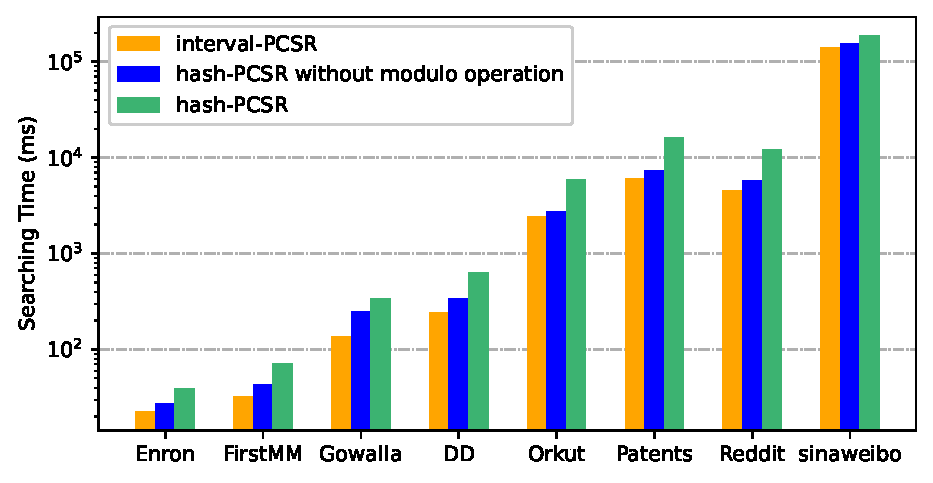
\includegraphics[width=\columnwidth]{./figure/accesstime.eps}
\caption{The searching time of interval- and hash-PCSR on all data graphs.}	
\label{fig:searchtime}
\end{figure}

We can see in Figure \ref{fig:searchtime} that our interval-PCSR achieves better performance than hash-PCSR in all data graphs and obtains
an average speedup of 2.4$\times$. In hash-PCSR, GSI first uses a hash function to calculate the index of a given VID, and then loads 32
indexes from global memory into shared memory. Finally, GSI finds the address of neighbors of the VID. Our approach needs to search the
given VID in intervals that are stored in shared memory and load the address of neighbors from global memory. Though our approach needs
more shared memory accesses than GSI, the accesses to shared memory in our interval-PCSR is aligned and the latency is negligible compared
to the global memory access. The main reason for the overhead of hash-PCSR is the calculation of hash indexes. More specifically, the
modulo operation in the hash function accounts for a large portion of execution time of the hash operation. We replace the variable divisor
of the modulo operation with a fixed constant and present the searching time in Figure \ref{fig:searchtime}. We can see that the hash-PCSR
runs much faster without the modulo operation. However, variable divisor is necessary for the modulo operation to generate correct results.

In summary, our interval-PCSR not only reduces the space cost of hash-PCSR by replacing hash indexes with interval indexes, but also
reduces the searching time by eliminating hash calculation.

\subsection{Comparison of \SystemName and GSI\label{sec:comparegsi}}
\begin{figure*}
\centering
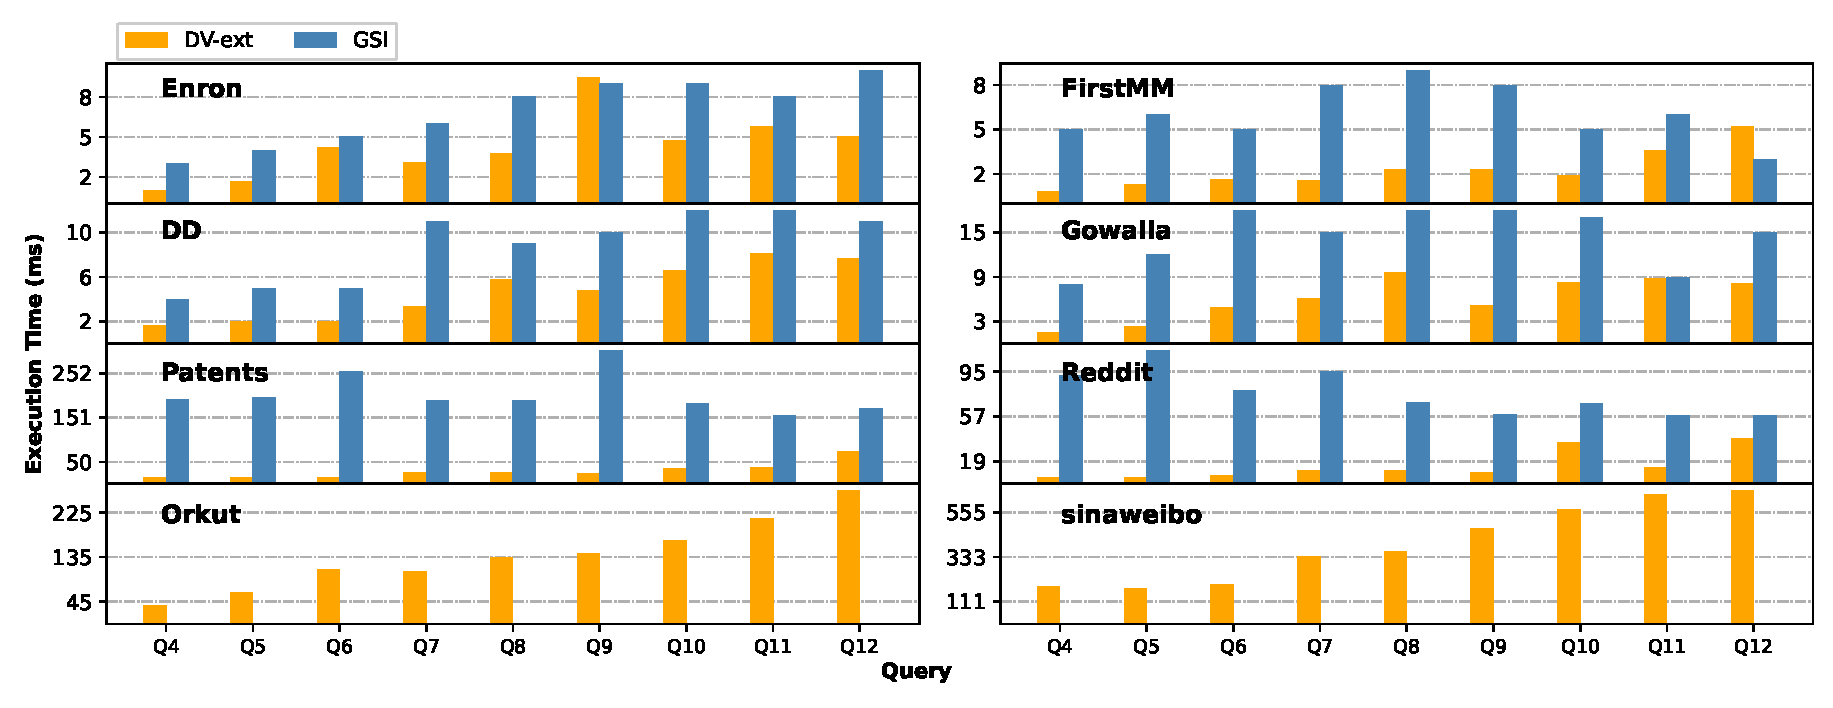
\includegraphics[width=\textwidth]{./figure/overperformance.eps}
\caption{Execution times of \SystemName and GSI for searching nine query graphs on each of eight data graphs.}	
\label{fig:overallperf}
\end{figure*}

\begin{figure}
\centering
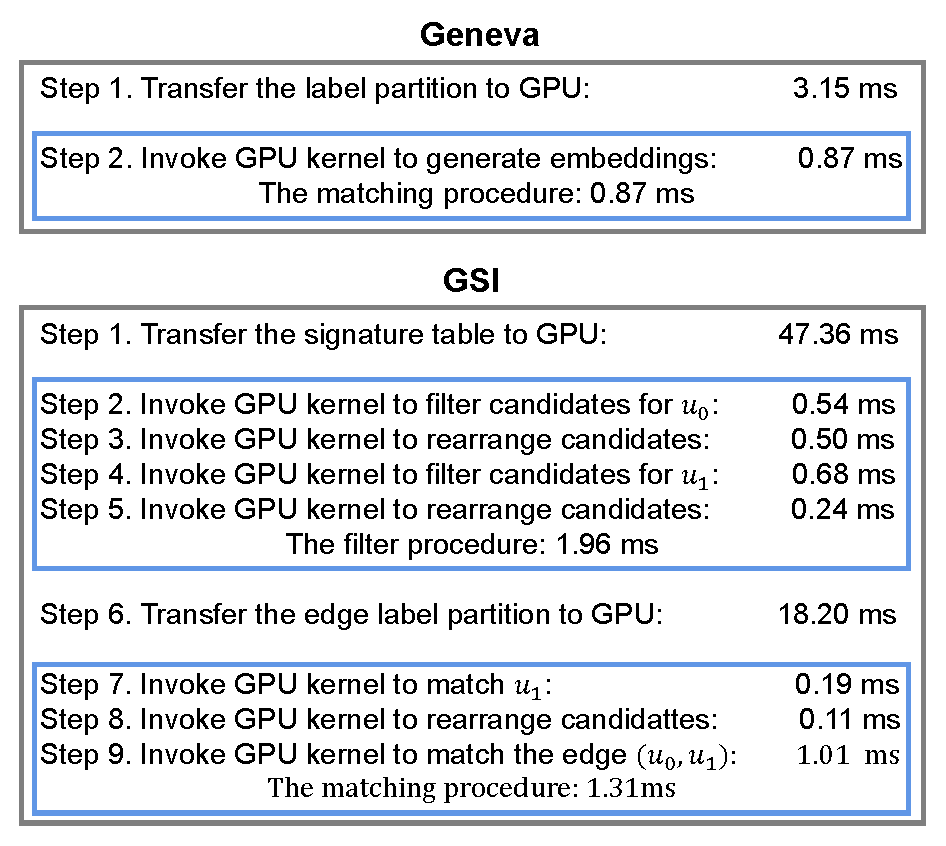
\includegraphics[width=\columnwidth]{./figure/comparegsi.eps}
\caption{The execution times of main procedures of \SystemName and GSI.}	
\label{fig:compdvgsi}
\end{figure}
In this section, we present the overall performance of \SystemName and GSI on eight data graphs. For each data graph, we first use random walk to extract nine query graphs from it with vertex count ranging from 4 to 12, and then employ both methods on the data graph to match the generated nine queries. The runtime results are shown in Fig \ref{fig:overallperf}. GSI runs out of GPU memory in data graphs Orkut and sinaweibo.

Our approach outperforms GSI in almost all test cases and achieves an average speedup of $5\times$. The maximum speedup of our approach over GSI can be up to $22.5\times$. As can be seen, GSI outperforms our approach in two test cases. The reasons can be explained as follows: (1) When matching $Q9$ in the data graph Enron, GSI finds 620K embeddings while \SystemName finds over 19M embeddings. GSI misses a vast number of embeddings, which makes it more faster than \SystemName; (2) When matching $Q12$ in the data graph FirstMM, GSI exits after matching three vertices because no embeddings can be matched, while \SystemName matches all vertices and edges of $Q12$ and finds one embedding. Therefore, \SystemName is slower than GSI in this test case.

In Figure \ref{fig:overallperf}, the average speedup of \SystemName over GSI is $7\times$ for small queries ($Q4$-$Q7$), while it is $3\times$ for large queries ($Q8$-$Q12$). The reason behind this phenomenon is explained as follows. \SystemName can generate an initial extension phase with at least two vertices. Additionally, if there exist vertices that form one of matching patterns 1-4, our approach can generate an initial extension phase with three vertices. Therefore, only two or three extension phases are needed for small queries to complete the matching process. This saves a large number of global memory accesses, which significantly accelerate the matching process for small query graphs.

To find out dominating factors for the superiority of \SystemName over GSI, we analyze detailed runtimes of each procedure of both methods. We employ \SystemName and GSI to match the query graph $Q4$ in the data graph Patents, and present the runtime of each step in Figure \ref{fig:compdvgsi}. We only show runtimes of procedures invoked when matching the first two query vertices, $u_0$ and $u_1$. The reasons are twofold: (1) In GSI, steps after matching $u_0$ and $u_1$ repeat steps 6-9 of Figure \ref{fig:compdvgsi}, and exhibit similar performance; (2) The runtimes of following steps are affected by the number of intermediate embeddings. Only when matching the first two vertices, we can make sure that both \SystemName and GSI process the same number embeddings.

We show the runtimes of \SystemName and GSI in Figure \ref{fig:compdvgsi}, and reveal three root causes of inefficiency of GSI compared to \SystemName.
\begin{itemize}
  \item GSI utilizes a filter procedure to prune candidates for each query vertex. It takes 1.96 ms to complete, which is twice the runtime of the matching procedure of \SystemName. Moreover, GSI needs to transfer the signature table to GPU before running the filter procedure. The runtime of data transfer along takes up 68\% runtime of GSI. This is because the signature table uses 64 bytes for each vertex in the data graph to store neighbor information, which results in a large data structure. Compared to GSI, \SystemName does not employ the filter procedure due to its inefficiencies in time and space.

  \item Before the matching procedure, both methods need to transfer the edge label partition to GPU. However, the execution time of data transfer in GSI is six times slower than \SystemName. The reason is explained as follows. GSI builds a hash-PCSR data structure for each edge label partition and inserts 30 empty entries into hash indexes to reduce the number of collisions. Consequently, hash-PCSR occupies a large portion of memory space, and thus takes a much longer time to be moved to GPU than the interval-PCSR of \SystemName.

  \item In the matching procedure, GSI invokes three GPU kernels to match the query vertex $u_1$, rearrange intermediate embeddings, and match the edge between $u_0$ and $u_1$, respectively. The kernel invoked in step 9 consumes most of the runtime of the matching procedure because it uses multiple time-consuming operations, such as thread block level synchronization and memory copy operations, inside the GPU kernel to maintain load balance. The four-layer load balance scheme of GSI can reduce the load imbalance greatly but also incur significant overhead. Different from GSI, our load balance scheme is simple yet effective. Only when there is no embeddings left, load imbalance can occur.
\end{itemize}

In summary, our approach obtains superior performance over GSI which is the state-of-the-art subgraph matching approach on GPU.

\subsection{Comparison of \SystemName and SV-match} \label{sec:comparesv}
\begin{figure*}
\centering
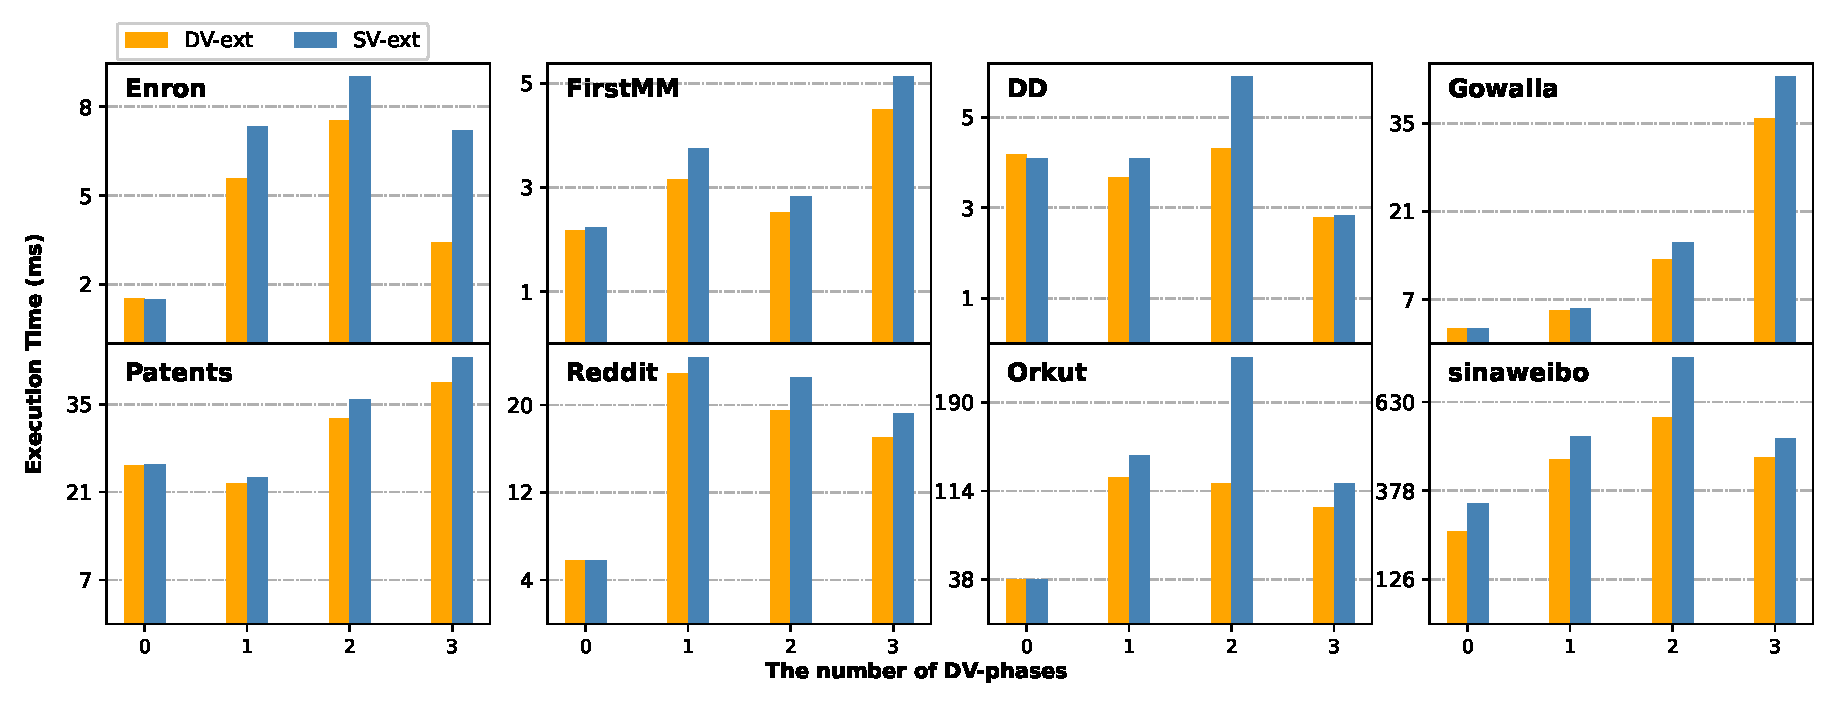
\includegraphics[width=\textwidth]{./figure/compareSV.eps}
\caption{Execution times of \SystemName and SV-match for different number of extension phases that contain matching patterns 1-7.}	
\label{fig:compareSV}
\end{figure*}
To further evaluate the performance of \SystemName, we demonstrate how the number of extension phases that contain matching patterns 1-7 affect the performance of \SystemName. For simplicity, we call the extension phase that contains one of matching patterns 1-7 the PV-phase, and the extension phase that contains the matching pattern 0 the SV-phase. For each data graph, we use random walk to extract several query graphs and classify them into different categories by the number of PV-phase, and select one query graph from each category for each data graph. The results are shown in Figure \ref{fig:compareSV}.

We can see in Figure \ref{fig:compareSV} that when the number of PV-phase is 0, both \SystemName and SV-match exhibit similar performance because all phases of both methods are the same. When the number of pV-phase is 1, 2, and 3, \SystemName improves the performance of SV-match by 11.3\%, 20.2\%, and 16.3\% respectively. In the data graph DD, the performance of \SystemName is very close to SV-match because there is only one embedding that is isomorphic to the query graph and the runtime is too short to observe the difference between \SystemName and SV-match.

\section{Discussions}
Naturally, there is room for further work and improvement. We discuss a few points there.

\cparagraph{Matching more than two vertices.} \FIXME{XX}

\cparagraph{Other discussions.}

\section{Related Work}
\subsection{CPU-based Subgraph Search}
An early attempt for subgraph search is Ullmann \cite{ullmann1976algorithm}, which uses a tree-search based approach to mine subgraphs. Many works \cite{cordella2001improved, shang2008taming,zhang2009gaddi,he2008graphs,zhao2010graph} based on Ullmann have been proposed. VF2 \cite{cordella2001improved} and QuickSI \cite{shang2008taming} utilize vertex and edge information to eliminate invalid embeddings. GADDI \cite{zhang2009gaddi}, GraphQL \cite{he2008graphs}, and SPath \cite{zhao2010graph} utilize the neighborhood information to remove unqualified data vertices from the candidate set for each query vertex. CECI \cite{bhattarai2019ceci} proposes a compact embedding cluster index to divide the data graph into embedding clusters and conduct subgraph matching on each embedding cluster.

Subsequent works \cite{han2013turboiso,ren2015exploiting,bi2016efficient,han2019efficient,rivero2017efficient} try to build auxiliary data to devise an effective matching order. TurboIso \cite{han2013turboiso} first identifies candidate regions in a data graph and then generates a matching order for each candidate region based on the number of candidate vertices of query vertices in this candidate region. CFL \cite{bi2016efficient} decomposes the query graph into the core-forest-leaf structure and matches the core structure first to eliminate invalid embeddings as early as possible. SGMatch \cite{rivero2017efficient} decomposes the query graph into graphlets and then generates a matching order based on graphlets. Distributed subgraph search has been explored in \cite{afrati2013enumerating, shao2014parallel,shi2020graphpi,talukder2016distributed,sun2018parallelizing,plantenga2013inexact,reza2018prunejuice}. These approaches use MPI and MapReduce to distribute subgraph search tasks to different compute nodes.

Different from CPU-based approaches, our work focuses on exploiting a GPU's massive parallelism to match a query graph in a data graph.

\subsection{GPU-based Subgraph Search}
GPU has been used to accelerate applications in many fields because of its massive parallelism. There are several works exploiting GPU acceleration for subgraph search. TRICORE \cite{hu2018tricore}  and \cite{green2014fast} design a GPU-based triangle counting method. Guo at el. \cite{guo2020gpu} partitions the data graph that beyond the GPU memory into subgraphs and matches the query graph in each subgraph iteratively. They also propose an embedding reuse method to avoid repeated computation in the work \cite{guo2020exploiting}. GSI \cite{zeng2020gsi}, GSM \cite{wang2020fast}, GpSM \cite{tran2015fast}, and \cite{lin2016network} utilize auxiliary data to assist candidate pruning and some GPU-based optimization techniques to speed up the matching process. While these works adopt the single vertex matching method, our approach uses parallel vertex matching method to reduce the number of read and write operations of  embeddings.



\section{Conclusions}
In this work, we propose a parallel vertex matching method to match query graphs in a labeled undirected data graph. Also, we improve the performance of hash-PCSR by replacing its hash indexes with interval indexes. Experiments show that our approach consistently outperforms GSI, which is the state-of-the-art subgraph search method on GPU, in all tested data graphs. We also validate the effectiveness of parallel vertex matching method by comparing it to the single vertex matching method.

\bibliographystyle{ACM-Reference-Format}
\bibliography{refs}
\end{document}
\endinput
